\section{Agentic Scientific Figure and Visualization Generation}
\label{sec:scientific-visualization}

Scientific and data-grounded graphics bind visual communication to source fidelity. Here the artifact is simultaneously an image, a structured specification, an executable program, and an argument about data. Agentic control must therefore coordinate analytical intent, chart or diagram structure, code execution, visual inspection, and checks that the rendered claim remains supported by the source.

\begin{keytakeaway}[Agentic Scientific Visualization at a Glance]
\begin{keypoints}
  \item \textbf{Data-to-chart analysis and executable visualization:} translate analytical intent into data transformations, encodings, and executable plotting code, where execution catches syntax failures but factual and perceptual validity require further checks.

  \item \textbf{Scientific figures and diagrams:} add domain semantics, symbolic structure, and source-document grounding, keeping the state editable and traceable to evidence.

  \item \textbf{Rendered feedback, semantic validation, and benchmarks:} combine inverse parsing, code execution, rule checking, visual critique, and source consistency, showing both the strength of heterogeneous evidence and the remaining difficulty of converting a diagnosis into a correct local repair.
\end{keypoints}
\end{keytakeaway}

\begin{figure}[!htbp]
  \centering
  
\definecolor{avgmapblue}{HTML}{22558A}
\definecolor{avgmapgreen}{HTML}{23845D}
\ifdefined\avgmapfont\else\newcommand{\avgmapfont}{\rmfamily}\fi
\makebox[\linewidth][c]{%
\resizebox{0.98\linewidth}{!}{%
\begin{tikzpicture}[
  avg branch/.style={draw=avgmapblue!58, fill=avgmapblue!9, text=black!88, rounded corners=2.5pt, line width=0.48pt, text width=42mm, minimum height=10.5mm, align=center, inner xsep=2.2mm, inner ysep=0.9mm, outer sep=0pt, execute at begin node={\hyphenpenalty=10000\exhyphenpenalty=10000\relax}, font=\avgmapfont\fontsize{7.35}{8.35}\selectfont\bfseries},
  avg papers/.style={draw=avgmapblue!25, fill=avgmapblue!2, text=black!88, rounded corners=2.5pt, line width=0.38pt, text width=115mm, minimum height=10.5mm, align=left, inner xsep=3mm, inner ysep=0.9mm, outer sep=0pt, execute at begin node={\hyphenpenalty=10000\exhyphenpenalty=10000\relax}, font=\avgmapfont\fontsize{7.15}{8.25}\selectfont\bfseries},
  avg benchmark branch/.style={avg branch, draw=avgmapgreen!78, fill=avgmapgreen!15, text=avgmapgreen!45!black},
  avg benchmark papers/.style={avg papers, draw=avgmapgreen!72, fill=avgmapgreen!7, text=black!88},
  avg root/.style={draw=avgmapblue, fill=avgmapblue!94!black, text=white, rounded corners=2.5pt, line width=0.55pt, minimum width=9mm, minimum height=36mm, inner sep=0pt, outer sep=0pt},
  avg line/.style={draw=black!28, line width=0.45pt, line cap=round},
  avg benchmark line/.style={draw=avgmapgreen!78, line width=0.55pt, line cap=round}
]
\matrix (avgmap) [matrix of nodes, row sep=1.35mm, column sep=3mm, ampersand replacement=\&, nodes={anchor=center}] {
  \node[avg branch] (c7b1) {Executable Visualization}; \& \node[avg papers] (c7p1) {LightVA~\cite{zhao2024lightva}, MultiVis-Agent~\cite{avg260118320}, ChatVis~\cite{avg250723096}, PlotEdit~\cite{avg250111233}, GA-VisAgent~\cite{avg260501299}.}; \\
  \node[avg branch] (c7b2) {Figures and Diagrams}; \& \node[avg papers] (c7p2) {VisPainter~\cite{avg251027452}, SciFig~\cite{huang2026scifig}, EduVisAgent~\cite{avg250516832}, Feynman~\cite{avg260312597}, SASAV~\cite{avg260403406}.}; \\
  \node[avg branch] (c7b3) {Feedback and Validation}; \& \node[avg papers] (c7p3) {AMACE~\cite{namgoong2025amace}, PlotGen~\cite{goswami2025plotgen}, HiLSVA~\cite{avg260626614}, PMVisAgent~\cite{avg260529692}, SciVisAgentSkills~\cite{avg260605525}.}; \\
  \node[avg benchmark branch] (c7b4) {Benchmarks}; \& \node[avg benchmark papers] (c7p4) {VisBench~\cite{avg251027452}, SciFig-Bench~\cite{huang2026scifig}, SciFlow-Bench~\cite{avg260209809}, SciVisAgentBench~\cite{avg260329139}.}; \\
};
\coordinate (c7trunktop) at ($(c7b1.west)+(-4.6mm,0)$);
\coordinate (c7trunkbottom) at ($(c7b4.west)+(-4.6mm,0)$);
\coordinate (c7rootnw) at ($(c7b1.north west)+(-15.5mm,0)$);
\coordinate (c7rootse) at ($(c7b4.south west)+(-7.6mm,0)$);
\node[avg root, fit=(c7rootnw)(c7rootse)] (c7root) {};
\node[rotate=90, align=center, text=white, font=\avgmapfont\fontsize{7.05}{8.15}\selectfont] at (c7root.center) {{\bfseries CHAPTER 7}\\[0.55mm]{\fontsize{6.2}{7.15}\selectfont Scientific figures and visualization}};
\draw[avg line] (c7trunktop) -- (c7trunkbottom);
\coordinate (c7trunkmid) at ($(c7trunktop)!0.5!(c7trunkbottom)$);
\draw[avg line] (c7root.east) -- (c7trunkmid);
\draw[avg line] (c7trunktop |- c7b1.west) -- (c7b1.west);
\draw[avg line] (c7b1.east) -- (c7p1.west);
\draw[avg line] (c7trunktop |- c7b2.west) -- (c7b2.west);
\draw[avg line] (c7b2.east) -- (c7p2.west);
\draw[avg line] (c7trunktop |- c7b3.west) -- (c7b3.west);
\draw[avg line] (c7b3.east) -- (c7p3.west);
\draw[avg benchmark line] (c7trunktop |- c7b4.west) -- (c7b4.west);
\draw[avg benchmark line] (c7b4.east) -- (c7p4.west);
\end{tikzpicture}%
}%
}

  \caption{Representative systems and benchmarks for agentic scientific figure and visualization generation, organized according to the chapter taxonomy.}
  \label{fig:ch7-representative-systems}
\end{figure}

\subsection{Data-to-chart analysis and executable visualization.}
Chart agents translate analytical intent into data transformations, encodings, and executable plotting code. Execution catches syntax failures, but factual and perceptual validity require additional checks against the data and communicative goal.

\paragraph{LightVA}
 presents an LLM-agent framework that automates task planning, code generation, and linked visualization creation for exploratory visual analytics from raw datasets and high-level user goals~\cite{zhao2024lightva}. The framework (Planner, Executor, and Controller) supports human oversight through direct manipulation and natural language. Figure~\ref{fig:ch7-lightva} illustrates the visible analytical state and direct user controls exposed by the system.

\begin{figure}[!htbp]
  \centering
  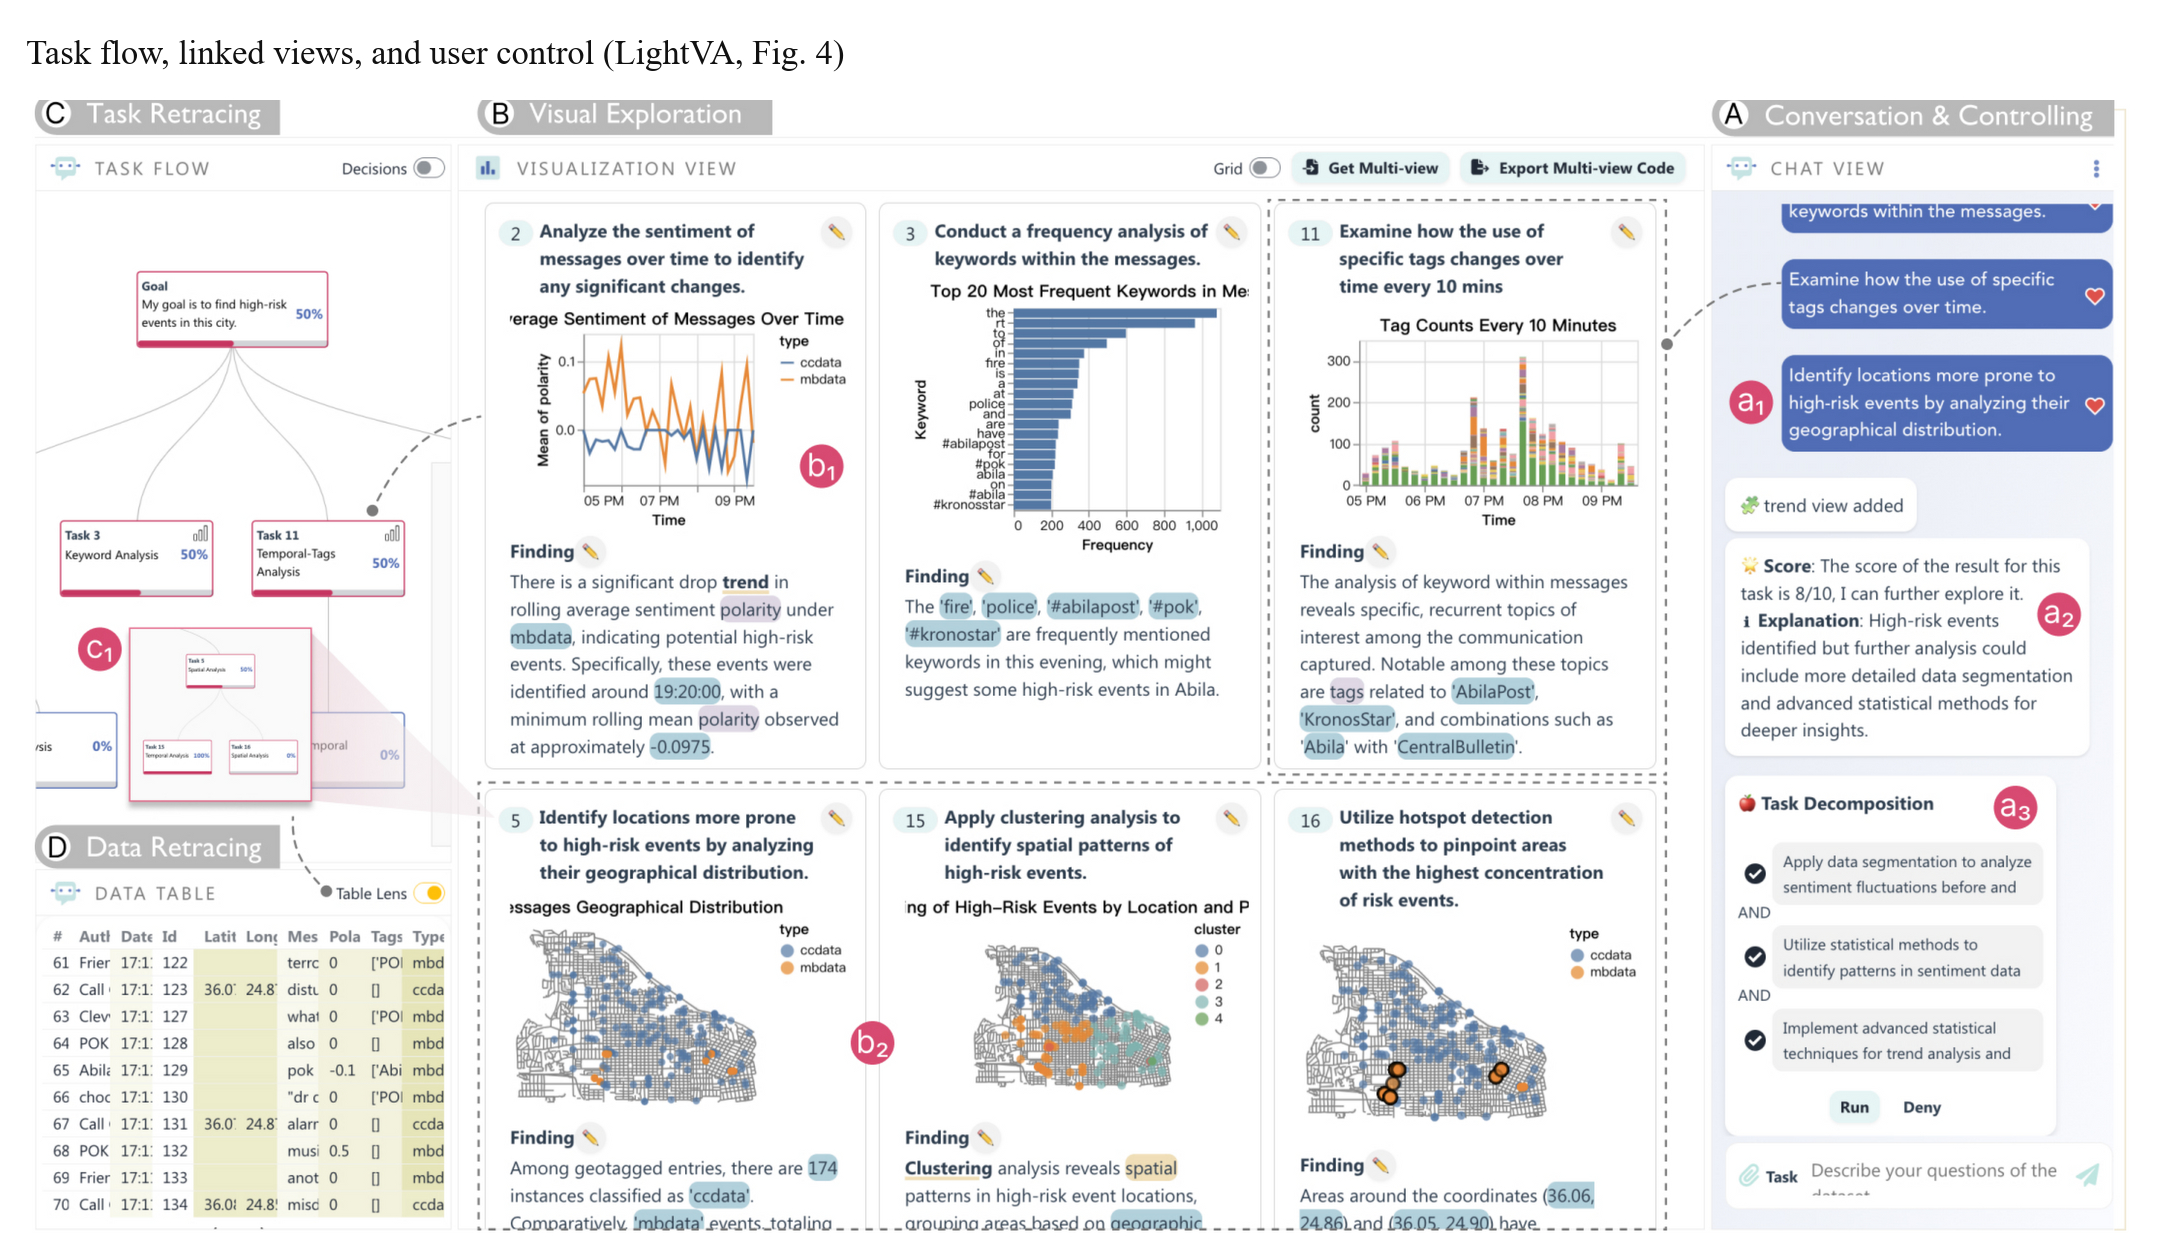
\includegraphics[width=\textwidth]{figures/ch7_executable_visual_analytics.jpg}
  \caption{Visible analytical state and user control in LightVA. The interface exposes the evolving task flow, linked data views, findings, and decomposition controls, allowing users to inspect and redirect executable visual analysis~\cite{zhao2024lightva}.}
  \label{fig:ch7-lightva}
\end{figure}

\paragraph{A2P-Vis}
 introduces a two-stage multi-agent pipeline that turns raw tabular data into a publication-ready data-visualization report containing executable charts, ranked insights, and narrative text~\cite{avg251222101}. The pipeline (Data Analyzer and Presenter) demonstrates end-to-end integration through a worked example without controlled evaluation of output quality.

\paragraph{MultiVis-Agent}
 presents a logic rule-enhanced multi-agent framework that extends text-to-chart generation to four scenarios—basic, image-referenced, code-referenced, and iterative refinement—with mathematical reliability guarantees~\cite{avg260118320}.

\paragraph{ChatVis}
is an LLM-based assistant that generates ParaView Python scripts for 3D and time-varying scientific visualization from natural language descriptions~\cite{avg250723096}. It combines chain-of-thought prompt decomposition, retrieval-augmented generation from a vector database of ParaView documentation and code examples, and iterative error correction that feeds execution failures back to the LLM until the code runs. Empirical evaluation on a benchmark of canonical tasks, regression tests, and scientific use cases demonstrates substantial improvements over unassisted state-of-the-art LLMs.


\paragraph{WaitGPT}
 is a prototype system that transforms LLM-generated data analysis code into an interactive flow diagram in real time, enabling users to monitor and steer conversational data analysis without deciphering raw code~\cite{avg240801703}. It parses scripts into visual operation chains with runtime table states and supports node-based inspection and refinement. User studies demonstrate reduced cognitive load and improved error detection over code-only interfaces.

\paragraph{Does It Run and Is That Enough?}
This study re-examines text-to-chart generation, questioning whether execution success alone suffices as evidence of chart quality and accessibility~\cite{avg250606175}.  A lightweight two-agent pipeline with interpreter-feedback-driven repair substantially reduces runtime errors on standard benchmarks, yet accessibility analysis reveals that most generated charts fail basic colorblindness criteria and manual review identifies hallucinations even in executable outputs. The paper argues that execution is largely solved and calls for shifting evaluation focus toward semantic fidelity, visual clarity, and accessibility.

\paragraph{METAL}
 introduces a vision-language model based multi-agent framework that generates chart code from reference images through iterative collaboration among generation, visual critique, code critique, and revision agents~\cite{li2025metal}. The visual critic diagnoses appearance discrepancies between rendered and reference charts, while the code critic identifies implementation defects; their feedback drives iterative refinement until a quality threshold or compute budget is met.

\paragraph{PlotEdit}
 introduces a multi-agent framework for natural-language-driven editing of chart images in PDFs or scanned documents where source data and rendering code are unavailable~\cite{avg250111233}. Five specialized agents extract data tables, visual attributes, and code from the input chart, decompose user editing requests into executable steps, and implement modifications, coordinated through numeric, visual, and code feedback signals that iteratively rectify de-rendering errors. A perceptual fidelity feedback mechanism further ensures that only user-specified changes are applied while preserving unchanged chart components.

\paragraph{Exploring Agentic Workflows for Generating High Quality Math Visual Aids}
This study explores an agentic workflow for generating TikZ-based K-12 math diagrams through a QA-driven self-improvement loop~\cite{avg260709839}. A Diagram Generator produces initial TikZ code, a QA Generator formulates open-ended questions about accuracy and clarity, a QA Evaluator answers them using both code and rendered image, and a Verifier converts failed items into feedback for regeneration.

\paragraph{GA-VisAgent}
 is a multi-agent framework that translates geometric algebra formulas into executable GAALOPScript code and interactive 3D visualizations for educational purposes~\cite{avg260501299}. A ReAct-based Planner decomposes input formulas into categorized subtasks, which are routed to specialist agents for code generation, assignment, and visualization, while a validation agent checks syntax and triggers regeneration on failure.

\paragraph{Toward AI VIS Co-Scientists}
This work presents an end-to-end agentic harness that autonomously designs interactive scientific-visualization applications (VIS Apps) from raw datasets and high-level research tasks, producing linked views, filters, and analytical panels rather than static charts~\cite{avg260521825}. A primary code agent orchestrates exploratory data analysis, environment setup, planning, visualization implementation, and Playwright-based browser validation; evaluation reports drive iterative repair until blocking conditions are resolved, with project artifacts retained for traceability. 

\subsection{Scientific figures and diagrams.}
 add domain semantics, symbolic structure, and source-document grounding. Their state must remain editable and traceable to evidence, not merely visually similar to a target style.

\paragraph{From Pixels to Paths}
VisPainter is a multi-agent framework that converts natural language instructions into editable vector scientific diagrams by directly operating standard graphics software, keeping modules, connectors, and labels independently modifiable after generation~\cite{avg251027452}. A Manager orchestrates the workflow, a Designer proposes layouts and refines them via screenshot feedback, and a Toolbox executes over thirty editing operations. The accompanying VisBench benchmark provides 360 high-information-density diagrams with seven-dimensional metrics spanning content, layout, readability, and interaction cost.

\paragraph{SciFig}
 is a multi-agent framework that generates visually rich, fully editable methodology figures from scientific text, with four agents handling planning, layout, component rendering, and iterative refinement~\cite{huang2026scifig}. The output XML preserves individual blocks, arrows, and labels for post-hoc editing in standard tools. And SciFig-Bench provides 435 human-verified methodology figures across 37 AI/ML domains. 

\paragraph{EduVisAgent}
 is a multi-agent framework that generates pedagogical visual explanations for K-12 STEM problems, producing diagrams or interactive web pages that expose reasoning sequences and connect textual steps with visual elements~\cite{avg250516832}. A planning agent coordinates five specialized roles—conceptual mapping, reasoning decomposition, learning guidance, metacognitive prompting, and visualization design—to construct a pedagogical plan for rendering. EduVisBench provides 1,154 STEM questions across three subjects and 15 domains.

\paragraph{See it. Say it. Sorted}
This system converts hand-drawn sketches into editable SVG flow diagrams through an iterative critic–candidates–judge loop~\cite{avg250815222}. A Critic VLM compares the sketch with the current SVG and suggests qualitative relational edits; multiple LLMs generate diverse candidate SVG modifications; a Judge VLM selects the best candidate, reverting to the prior version if none improves and feeding back the failure.

\paragraph{Crafter}
 is a multi-agent harness that generates scientific figures across academic, poster, and infographic types from diverse inputs, and converts raster outputs into editable SVGs via CRAFTEDITOR~\cite{avg260530611}. A designer proposes candidate plans, an executor renders them, a critic diagnoses errors across six quality dimensions, and a reviser applies structured edits to a shared specification, with rollback to the best version when modifications degrade quality. CRAFTBENCH provides 279 samples across three figure types and four input conditions.

\paragraph{Feynman}
 is an LLM agent that generates knowledge-infused scientific diagrams at scale by decoupling knowledge elicitation from visual production~\cite{avg260312597}. It enumerates domain-specific ideas, plans Penrose programs, compiles them, and iteratively refines outputs via a panel of visual judges until quality thresholds are met; Penrose's optimization-based rendering ensures visual diversity while preserving semantics. And the Diagramma benchmark provides 1,058 questions across six subjects.

\paragraph{SASAV}
 is a fully autonomous multi-agent system that generates scientific visualizations from volumetric data without prior knowledge or human-in-the-loop feedback~\cite{avg260403406}. It profiles input data, retrieves domain knowledge via web search and RAG, recommends transfer functions through parallel MLLM-based evaluation of isosurfaces, and selects optimal viewpoints and exploratory trajectories—producing static images, animations, and interactive visualizations. The system operates as a fixed four-stage pipeline with batched MLLM inference.  

\subsection{Rendered feedback, semantic validation, and benchmarks.}
Evaluation in this domain can combine inverse parsing, code execution, rule checking, visual critique, and source consistency. The following work shows both the strength of heterogeneous evidence and the remaining difficulty of converting a diagnosis into a correct local repair.

\paragraph{AMACE}
 iteratively refines table-to-chart generation through a multi-agent loop without manual prompt engineering~\cite{namgoong2025amace}. A Code Generator produces Python code, a Renderer executes it, a multimodal Replier answers queries from the chart, and an Evaluator checks correctness against the table—feeding feedback back to the generator. An Early Stopping Checker terminates when quality criteria are met.



\paragraph{MAGMA-Edu}
 is a multi-agent framework that generates K-12 math problems with coherent text-diagram pairs through a two-stage generate–validate–reflect pipeline~\cite{avg251118714}. Stage 1 refines textual content via Generator, Validator, and Reflector agents; Stage 2 translates verified descriptions into executable Matplotlib code, rendered and iteratively corrected by Code Executor, Image Validator, and Image Reflector agents. The code-based intermediate representation ensures geometric fidelity and deterministic re-rendering after errors. 


\paragraph{PlotGen}
 is a multi-agent framework that generates scientific charts from natural language requests and data through iterative multimodal feedback~\cite{goswami2025plotgen}. A Query Planning Agent decomposes user requests, a Code Generation Agent produces Python code, and Numeric, Lexical, and Visual Feedback Agents inspect the rendered chart—verifying data trends, textual labels, and visual aesthetics—and return diagnoses to revise the code. 

\paragraph{HiLSVA}
 is a human-in-the-loop agentic system that supports mixed-initiative scientific visualization workflows in ParaView through plan-first execution, stepwise provenance tracking, and test-time adaptation~\cite{avg260626614}. An orchestrator coordinates specialized agents; users can co-plan, approve actions, directly manipulate visualizations, and restore prior states, while a self-improving agent reflects on outcomes, queries users when uncertain, and stores validated knowledge for reuse.

\paragraph{Perceptual Self-Reflection}
This framework generates physics simulation code from natural language and validates it through perceptual self-reflection: rendering the animation, sampling frames, and using a vision-language model to check physical criteria—routing diagnoses to requirement or code revision~\cite{avg260212311}. Iteration continues until quality thresholds are met or ten attempts are exhausted. 

\paragraph{Progressive Text-to-Visualization}
This paper introduces a progressive multi-turn text-to-visualization paradigm where users iteratively refine queries and each turn yields executable VQL, along with PMVisBench for evaluation and PMVisAgent for execution~\cite{avg260529692}. PMVisBench is constructed by reverse-simplifying complete VQLs with constraints to ensure intermediate validity. PMVisAgent employs three agents with ReAct-style validation tools to detect and repair errors before propagating to the next round, significantly outperforming one-shot baselines.

\paragraph{Agentic Visualization}
This paper presents 11 design patterns for agentic visualization—systems that integrate autonomous agents while preserving human analytical control—extracted from prior visualization literature~\cite{avg250519101}. The patterns span Agent Roles (Forager, Analyst, Chart Creator, Storyteller), Communication (Insight Timeline, Progress Indicator, Provenance Log), and Coordination (Scouting, Swarming, Monitoring, Consolidating), each specifying problem, solution, examples, and tradeoffs. The catalog is validated through examples and a composite scenario, providing a design vocabulary for future agentic visualization systems.

\paragraph{An Evaluation-Centric Paradigm for Scientific Visualization Agents}
This position paper advocates for systematic evaluation benchmarks for SciVis agents, proposing a dual framework of outcome-based and process-based evaluation organized around accuracy, coverage, and cost-effectiveness~\cite{avg250915160}. Outcome-based assessment uses MLLM judges for final visualization quality; process-based assessment examines intermediate actions via hard-coded state verifiers, token usage, and runtime. 

\paragraph{Exploring LLM Agent Designs and Interaction Modalities for Scientific Visualization}
This study compares domain-specific, general-purpose coding, and GUI-based agents on 15 ParaView tasks~\cite{avg260427996}. General-purpose coding agents achieve highest completion but at higher cost; domain-specific agents are more efficient yet less flexible. Persistent memory improves performance, and stepwise decomposition raises GUI agent pass rates to 60-65\%, indicating multi-step planning as the primary bottleneck.

\paragraph{SciFlow-Bench}
 evaluates scientific diagram generation by inverse-parsing pixel outputs into graphs, measuring structural recoverability rather than visual similarity~\cite{avg260209809}. A multi-agent pipeline constructs canonical graphs from source figures and reverse-parses generated images into predicted graphs for comparison. The benchmark contains 500 diagrams across five domains; among evaluated generators, Gemini 3 Pro Image achieves the highest aggregate score, yet substantial structural loss remains.

\paragraph{SciVisAgentBench}
 is a reproducible benchmark for evaluating LLM-based agents on scientific visualization tasks, grounded in a taxonomy of domains, data types, complexity, and operations~\cite{avg260329139}. It comprises 108 expert-authored cases evaluated through an outcome-centric pipeline combining LLM judgment with deterministic checks.A validity study with 12 experts shows Claude Opus 4.6 correlates at 0.806 with human judgments, supporting scalable assessment.

\paragraph{SciVisAgentSkills}
 is a collection of reusable procedural skills that equip general-purpose coding agents with tool-specific knowledge for ParaView, napari, VMD, and TTK workflows~\cite{avg260605525}. Each skill encodes environment assumptions, API patterns, examples, and heuristics as a static instruction package loaded at inference time without model retraining. Evaluated on SciVisAgentBench, skills improve mean task scores across most suites—e.g., Claude Code's ParaView score rises from 62.57 to 73.93—though effects vary by agent and task, and token usage does not consistently decrease.

Executable code and structured specifications make scientific graphics comparatively auditable, but not automatically truthful. Reliable control requires provenance from source to transformation to mark, plus visual and semantic checks that can identify the responsible stage when the final claim is wrong.

\FloatBarrier
